\documentclass[11pt]{jsarticle}
\usepackage{amsmath,amssymb}
\usepackage[dvipdfmx]{graphicx}
\usepackage[dvipdfmx]{color}
\usepackage{ascmac}
\usepackage{multirow}
\usepackage{geometry}    %余白調整
    \geometry{left=20mm,right=20mm,top=20mm,bottom=20mm}
\usepackage{caption}
    \captionsetup[figure]{labelsep=space, font={sf, small}}    %コロンを消す,小さめゴシック体
    %\captionsetup[table]{labelsep=space, font={sf, small}, justification=raggedright, singlelinecheck=off}
\usepackage[subrefformat=parens]{subcaption}
\usepackage{dcolumn}    %小数点揃え
\usepackage{fancybox}    %枠で囲む
\usepackage{siunitx}    %単位
\usepackage{mhchem}    %化学式
\usepackage{times}    %英数字font指定
\usepackage{titlesec}   %セクションタイトル定義
\usepackage{fancyhdr}   %ヘッダーおよびフッターの編集
\usepackage{cite}  % 文献引用のため
%
\renewcommand{\figurename}{Fig.~}
\renewcommand{\tablename}{Table~}
%
\DeclareSIUnit{\mM}{\si{\milli M}}  %mM
%
%%%%%セクションタイトルの文字サイズ指定%%%%%
\titleformat*{\section}{\bfseries}
\titleformat*{\subsection}{\bfseries}

%%%%ヘッダとフッタの指定%%%%
\pagestyle{fancy}
\renewcommand{\headrulewidth}{0pt} % ヘッダの線を消す
\lhead{{\footnotesize サンプルヘッダ 2024/01/01}} %ヘッダの左側
%\chead{\Large{}} %ヘッダの中央
\rhead{{\footnotesize 著者名}} %ヘッダの右側
%\lfoot{} %フッタの左側
%\cfoot{} %フッタの中央
%\rfoot{} %フッタの右側

\begin{document}

\begin{flushleft}   %title
  \textbf{サンプルレポート}\\
\end{flushleft}

\section{パッケージを使用したサンプル}
\subsection{はじめに}  %はじめに
この文書は,さまざまな{\LaTeX}パッケージを使用して作成したサンプルです.
数式、図、表、および化学式の使用例を示します.

\subsection{数式}  %amsmath

\texttt{amsmath}パッケージを使用した基本的な数式の例を示します.
\begin{equation}
  E = mc^2
\end{equation}

\subsection{図} %graphicx, caption
次に、\texttt{graphicx}および\texttt{caption}パッケージを使用した図の挿入方法を示します.

日本語のファイル名にも対応しています.

\begin{figure}[h]
    \centering
    \begin{subfigure}[b]{0.4\textwidth}
        \centering
        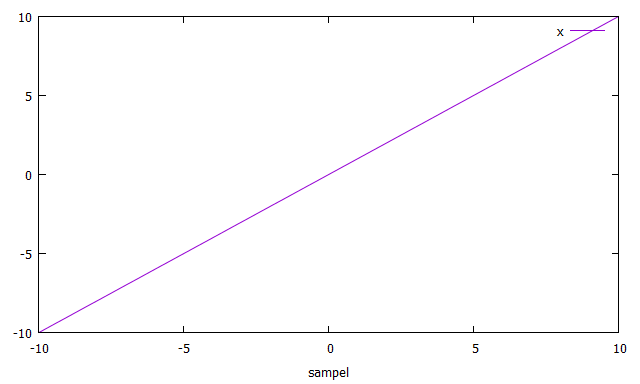
\includegraphics[width=\textwidth]{figure/sample.png}
        \caption{PNG}
        \label{fig:sample-png}
    \end{subfigure}
    \hfill
    \begin{subfigure}[b]{0.4\textwidth}
        \centering
        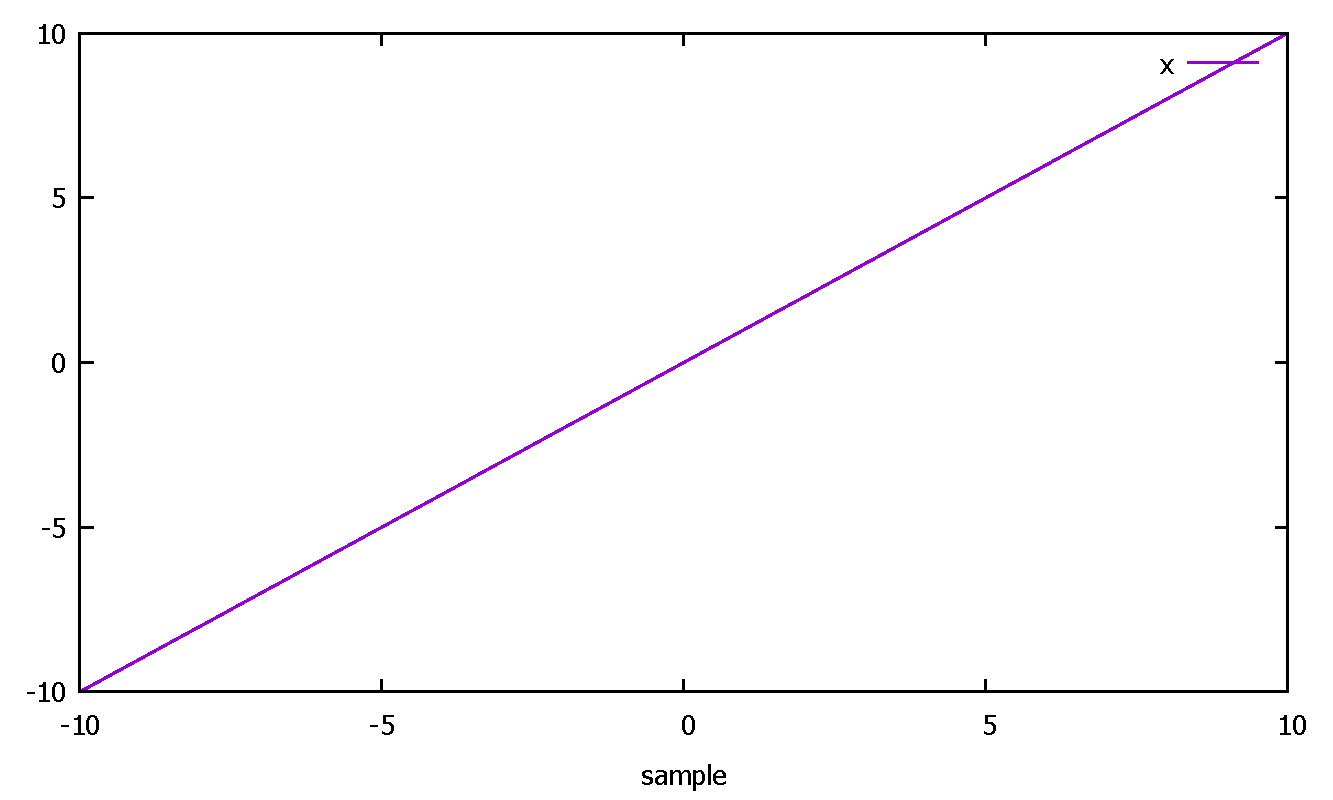
\includegraphics[width=\textwidth]{figure/sample.pdf}
        \caption{PDF}
        \label{fig:sample-pdf}
    \end{subfigure}

    \vspace{1em}

    \begin{subfigure}[b]{0.4\textwidth}
        \centering
        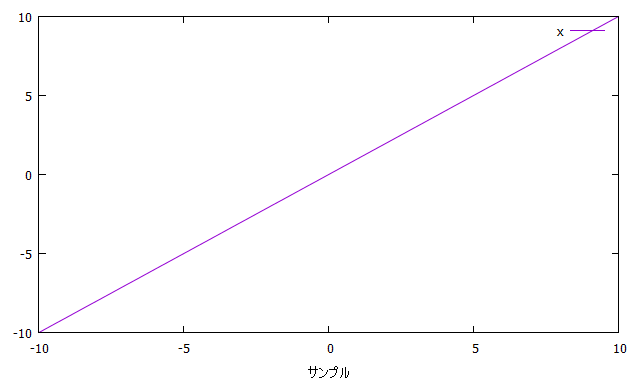
\includegraphics[width=\textwidth]{figure/サンプル.png}
        \caption{日本語 PNG}
        \label{fig:sample-png-ja}
    \end{subfigure}
    \hfill
    \begin{subfigure}[b]{0.4\textwidth}
        \centering
        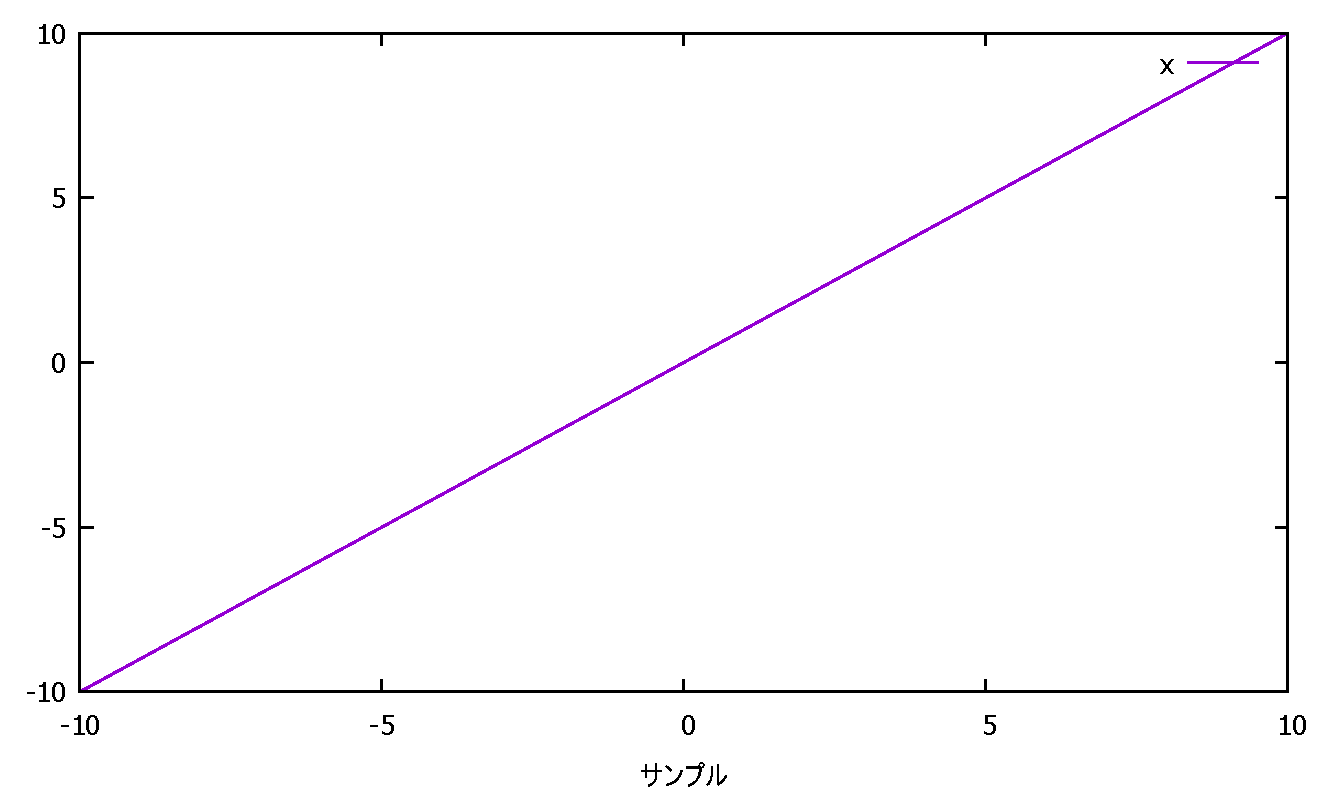
\includegraphics[width=\textwidth]{figure/サンプル.pdf}
        \caption{日本語 PDF}
        \label{fig:sample-pdf-ja}
    \end{subfigure}
    
    \caption{英語と日本語のPNGおよびPDFサンプル画像}
    \label{fig:all-images}
\end{figure}

\clearpage

\subsection{表} %dcolumn

\texttt{dcolumn}パッケージを使用して、小数点で揃えた表の例を示します.

\begin{table}[h]
    \centering
    \caption{サンプル表}
    \begin{tabular}{|c|D{.}{.}{2}|}
        \hline
        \textbf{項目} & \textbf{値} \\
        \hline
        A & 12.34 \\
        B & 56.78 \\
        C & 90.12 \\
        \hline
    \end{tabular}
    \label{tab:sample}
\end{table}

\section{化学式} %mhchem

\texttt{mhchem}パッケージを使用して、化学反応式を以下のように記述できます.

\begin{equation}
    \ce{H2 + O2 -> H2O}
\end{equation}

\section{文献} %cite

文献は以下に示します。文献の例として、\cite{sample2024}と\cite{example2024}を参照しました.

\bibliographystyle{plain}  % 文献スタイルを指定
\bibliography{bibtex/sample}  % BibTeXデータベースファイルを指定

\section{おわりに} %おわりに

このサンプル文書では、いくつかの{\LaTeX}パッケージを使用して、レポートを作成する方法を示しました.

\end{document}
